
%(BEGIN_QUESTION)
% Copyright 2014, Tony R. Kuphaldt, released under the Creative Commons Attribution License (v 1.0)
% This means you may do almost anything with this work of mine, so long as you give me proper credit

Bruk Kirchhoffs spenningslov til å beregne størrelse og polaritet på spenningen over motstandene $R_2$ og $R_4$ i dette motstandsnettverket:

$$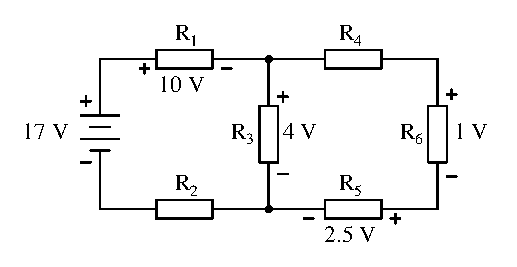
\includegraphics[width=15.5cm]{i01156x01.eps}$$

\underbar{file i01156}
%(END_QUESTION)





%(BEGIN_ANSWER)

$$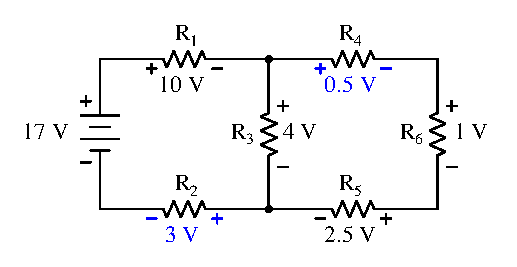
\includegraphics[width=15.5cm]{i01156x02.eps}$$

%(END_ANSWER)





%(BEGIN_NOTES)

I gjennomgangen bør dere undersøke mer enn én ``sløyfe'' når dere bruker KVL.  Det viser ikke bare at sløyfevalget i stor grad er vilkårlig, men fungerer også som en ekstra kontroll av arbeidet.

Det er ikke nødvendig å kunne serie-parallellkretser, eller engang parallellkretser, for å finne spenningen over $R_2$ og $R_4$ -- det holder å kunne bruke Kirchhoffs spenningslov.

%INDEX% Elektronikkrepetisjon: serie-parallellkretser

%(END_NOTES)

